\section{Distributed collaboration with GAP/Sage}\label{sec:gapsage}
\label{sec:handles}

Another aspect of interoperability in a mathematical VRE is the possibility of distributed
multisystem computations, where \emph{e.g.}\ a given system may decide to delegate
certain subcomputations or reasoning tasks to other systems.

There are already a variety of peer-to-peer interfaces between systems
in the \ODK project (see Figure~\ref{fig:interop}), which are based on
the \emph{handle paradigm}; for example \Sage includes, among others,
interfaces for \GAP, \Singular, and \Pari.
%
In this paradigm, when a system $A$ delegates a calculation to a system $B$, the
result $r$ of the calculation is not converted to a native $A$ object; instead $B$ just
returns a \emph{handle} $h$ (or reference) to the object $r$. Later $A$ can run further calculations
with $r$ by passing it as argument to functions or methods of $B$. The advantages of this
approach include that we can avoid the overhead of back and forth conversions between $A$
and $B$ and that we can manipulate objects of $B$ from $A$ even if they have no native
representation in $A$.

The next desirable feature is for the handle $h$ to behave in $A$ as
it was a native $A$ object; in other words, one wants to adapt the API
satisfied by $r$ in $B$ to mach the API for the same kind of objects
in $A$. For example, the method call \texttt{h.cardinality()} on a
\Sage handle \texttt{h} to a \GAP object \texttt{G} should trigger in
\GAP the corresponding function call \texttt{Size(G)}.

This can be implemented using the classical \emph{adapter
  pattern}, mapping calls to \Sage's method to corresponding \GAP
methods. \emph{Adapter classes} have already been implemented for
certain types of objects, like \Sage's \texttt{PermutationGroup} or
\texttt{MatrixGroup}. However this implementation lacks modularity:
for example, if \texttt{h} is a handle to a mere set \texttt{S}, \Sage
cannot use the \emph{adapter method} that maps
\texttt{h.cardinality()} to \texttt{Size(S)}, because this adapter
method is only available in the above two adapter classes.

To get around this problem we have worked on a more semantic
integration, where adapter methods are made aware of the type
hierarchies of the respective systems, and defined at the highest
available level of generality, as in Listing~\ref{lst:adapter}.
\begin{lstlisting}[language=Python,label=lst:adapter,
  caption=A semantic adapter method in \Sage]
class Sets: # Everything generic about sets in Sage
    class GAP: # Adapter methods relevant to Sets in the Sage-Gap interface
         class ParentMethods: # Adapter methods for sets
             def cardinality(self): # The adapter for the cardinality method
                 return self.gap().Size().sage()
         class ElementMethods: # Adapter methods for set elements
             ...
         class MorphismMethods: # Adapter methods for set morphisms
             ...
class Groups: # Everything generic about groups in Sage
     # This automatically includes features defined at a more general level
\end{lstlisting}

This peer-to-peer approach however does not scale up to a dozen of
systems. This is where the MitM paradigm comes to the rescue. With it,
the task is reduced to building interface theories and inter-views into
the core MitM ontology, in such a way that the adapter pattern can be
made generic in terms of the MitM ontology structure, without relying
on the concrete structure of the respective type systems. Then the
adapter methods for each peer-to-peer interface can be automatically
generated.
%
In our example, the adapter method for \texttt{cardinality} can be
constructed automatically as soon as the MitM inter-views link the
\texttt{cardinality} function in the \Sage interface theory on Sets
with the \texttt{Size} function in the corresponding interface theory
for \GAP.

We will now show first results of our experiments with interface
theories and inter-views, including several applications beyond the
generation of interface theories that support distributed computation
for \Sage and \GAP.

\subsection{Semantics in the \Sage category system}

The \Sage library includes 40k functions and allows for manipulating
thousands of different kinds of objects. As usual in such large
systems, it is critical for taming code bloat to
\begin{compactenum}[\em i\rm)]
\item identify the core concepts describing common behavior among the objects;
\item implement generic operations that apply on all objects having a given
  behavior, with appropriate specializations when performance calls for it;
\item design or choose a process for selecting the best implementation available when
  calling an operation on one or several objects.
\end{compactenum}

Following mathematical tradition and the precedent of the \Axiom,
\Fricas, or \MuPAD systems, \Sage has developed a
category-theory-inspired ``category system'', and found a way to
implement it on top of the underlying \Python object
system~\cite{Sage,Sage.Categories}. In short, a \defemph{category} specifies
the available \defemph{operations} and the \defemph{axioms} they satisfy.
%
This category system models taxonomic knowledge from mathematics
explicitly and uses it to support genericity, control the method
selection process, structure the code and documentation, enforce
consistency, and provide generic tests.

\ednote{NT: switch this example to (magmas, *)?}
\ednote{NT: it would be nice to include here the MMT formalization of
  Size/cardinality}
\begin{wrapfigure}r{8cm}\vspace*{-2.5em}
\begin{lstlisting}[language=Python,escapechar=!]
!\color{red}{@semantic(mmt="sets")}!
class Sets:
    class ParentMethods:
         !\color{red}{@semantic(mmt="card?card", gap="Size")}!
         @abstractmethod
         def cardinality(self):
             "Return the cardinality of ``self``"
\end{lstlisting}
\vspace*{-.5em}
\caption{An annotated category in \Sage}\label{fig:anncat}\vspace*{-1.5em}
\end{wrapfigure}
To generate interface theories from the \Sage category system, we are experimenting with a
system of annotations in the \Sage source files. Consider for instance the situtation in
Figure~\ref{fig:anncat} where we have annotated the \texttt{Sets()} category in \Sage
with \texttt{@semantic} lines that state correspondences to other interface theories. From
these the \Sage-to-MMT exporter can generate the respective interface theories and views.

In ongoing experiments, variants of the annotations are tested for
annotating existing categories without touching their source files and
providing the signature or the corresponding method names in other
systems when this information has not yet been formalized elsewhere.
% \ednote{POD: Would it be interesting to add a line about the constraints that are taken into consideration? For instance, the versioning of systems in parallel might become more problematic if it becomes so heavily interdependent}


\subsection{Exporting the \GAP knowledge: type system documentation}
\label{sec:gaptypes}

As in \Sage, the \GAP type system encodes a wealth of mathematical
knowledge, which can influence method selection. For example
establishing that a group is nilpotent will allow for more efficient
methods to be run for finding its centre. The main difference lies in
the method selection process. In \Sage the operations
implemented for an object and the axioms they satisfy are specified by
its class which, together with its super classes, groups syntactically
all the methods applicable in this context. In \GAP, this information
is instead specified by the truth-values of a collection of
independent \defemph{filters}, while the context of applicability is
specified independently for each method.
%
Breuer and Linton describe the \GAP type system in \cite{breuer-linton} and
the \GAP documentation \cite{GAP4} also contains extensive information on the types
themselves.

\begin{wrapfigure}r{6cm}\vspace*{-2em}
  \includegraphics[width=6cm]{gap-graph}\vspace*{-.5em}
  \caption{The \GAP Knowledge Graph.\label{fig:gap-graph}}\vspace*{-2em}
\end{wrapfigure}
\GAP allows some introspection of this knowledge after the system is loaded: the values of
those attributes and properties that are unknown on creation, can be computed on demand, and stored for later reuse.% without the need to be recomputed.

As a first step in generating interface theories for the MitM ontology, we have developed
tools to access mathematical knowledge encoded in \GAP, such as introspection inside a
running \GAP session, export to JSON to import to MMT, and export as a graph for
visualisation and exploration. These will become generally available in the next \GAP
release. The JSON output of the \GAP object system with default packages is currently
around 11 Megabytes and represents a knowledge graph with 540 vertices, 759 edges and 8 connected
components, (see Figures~\ref{fig:gap-graph},\ref{fig:gap-ismagma}). If all
packages are loaded, this graph expands to 1616 vertices, 2178 edges and 17 connected
components.

There is however another source of knowledge in the \GAP universe: the documentation, which is
provided in the GAPDoc format \cite{gapdoc}. Besides the main manuals, GAPDoc
is adopted by 97 out of the 130 packages currently redistributed with
GAP. Conventionally GAPDoc is used to build text, PDF and HTML versions of the manual
from a common source given in XML. The reference manual has almost 1400 pages and the
packages add hundreds more.

The GAPDoc sources classify documentation by the type of the documented object (function,
operation, attribute, property, etc.) and index them by system name. In this sense they
are synchronized with the type system (which \emph{e.g.}\ has the types of the functions) and can
be combined into flexiformal OMDoc/MMT interface theories, just like the ones for \LMFDB
in Section~\ref{sec:lmfdb}. This conversion is currently under development and will lead
to a significant increase of the scope of the MitM ontology. 

\begin{figure}[ht]\centering
  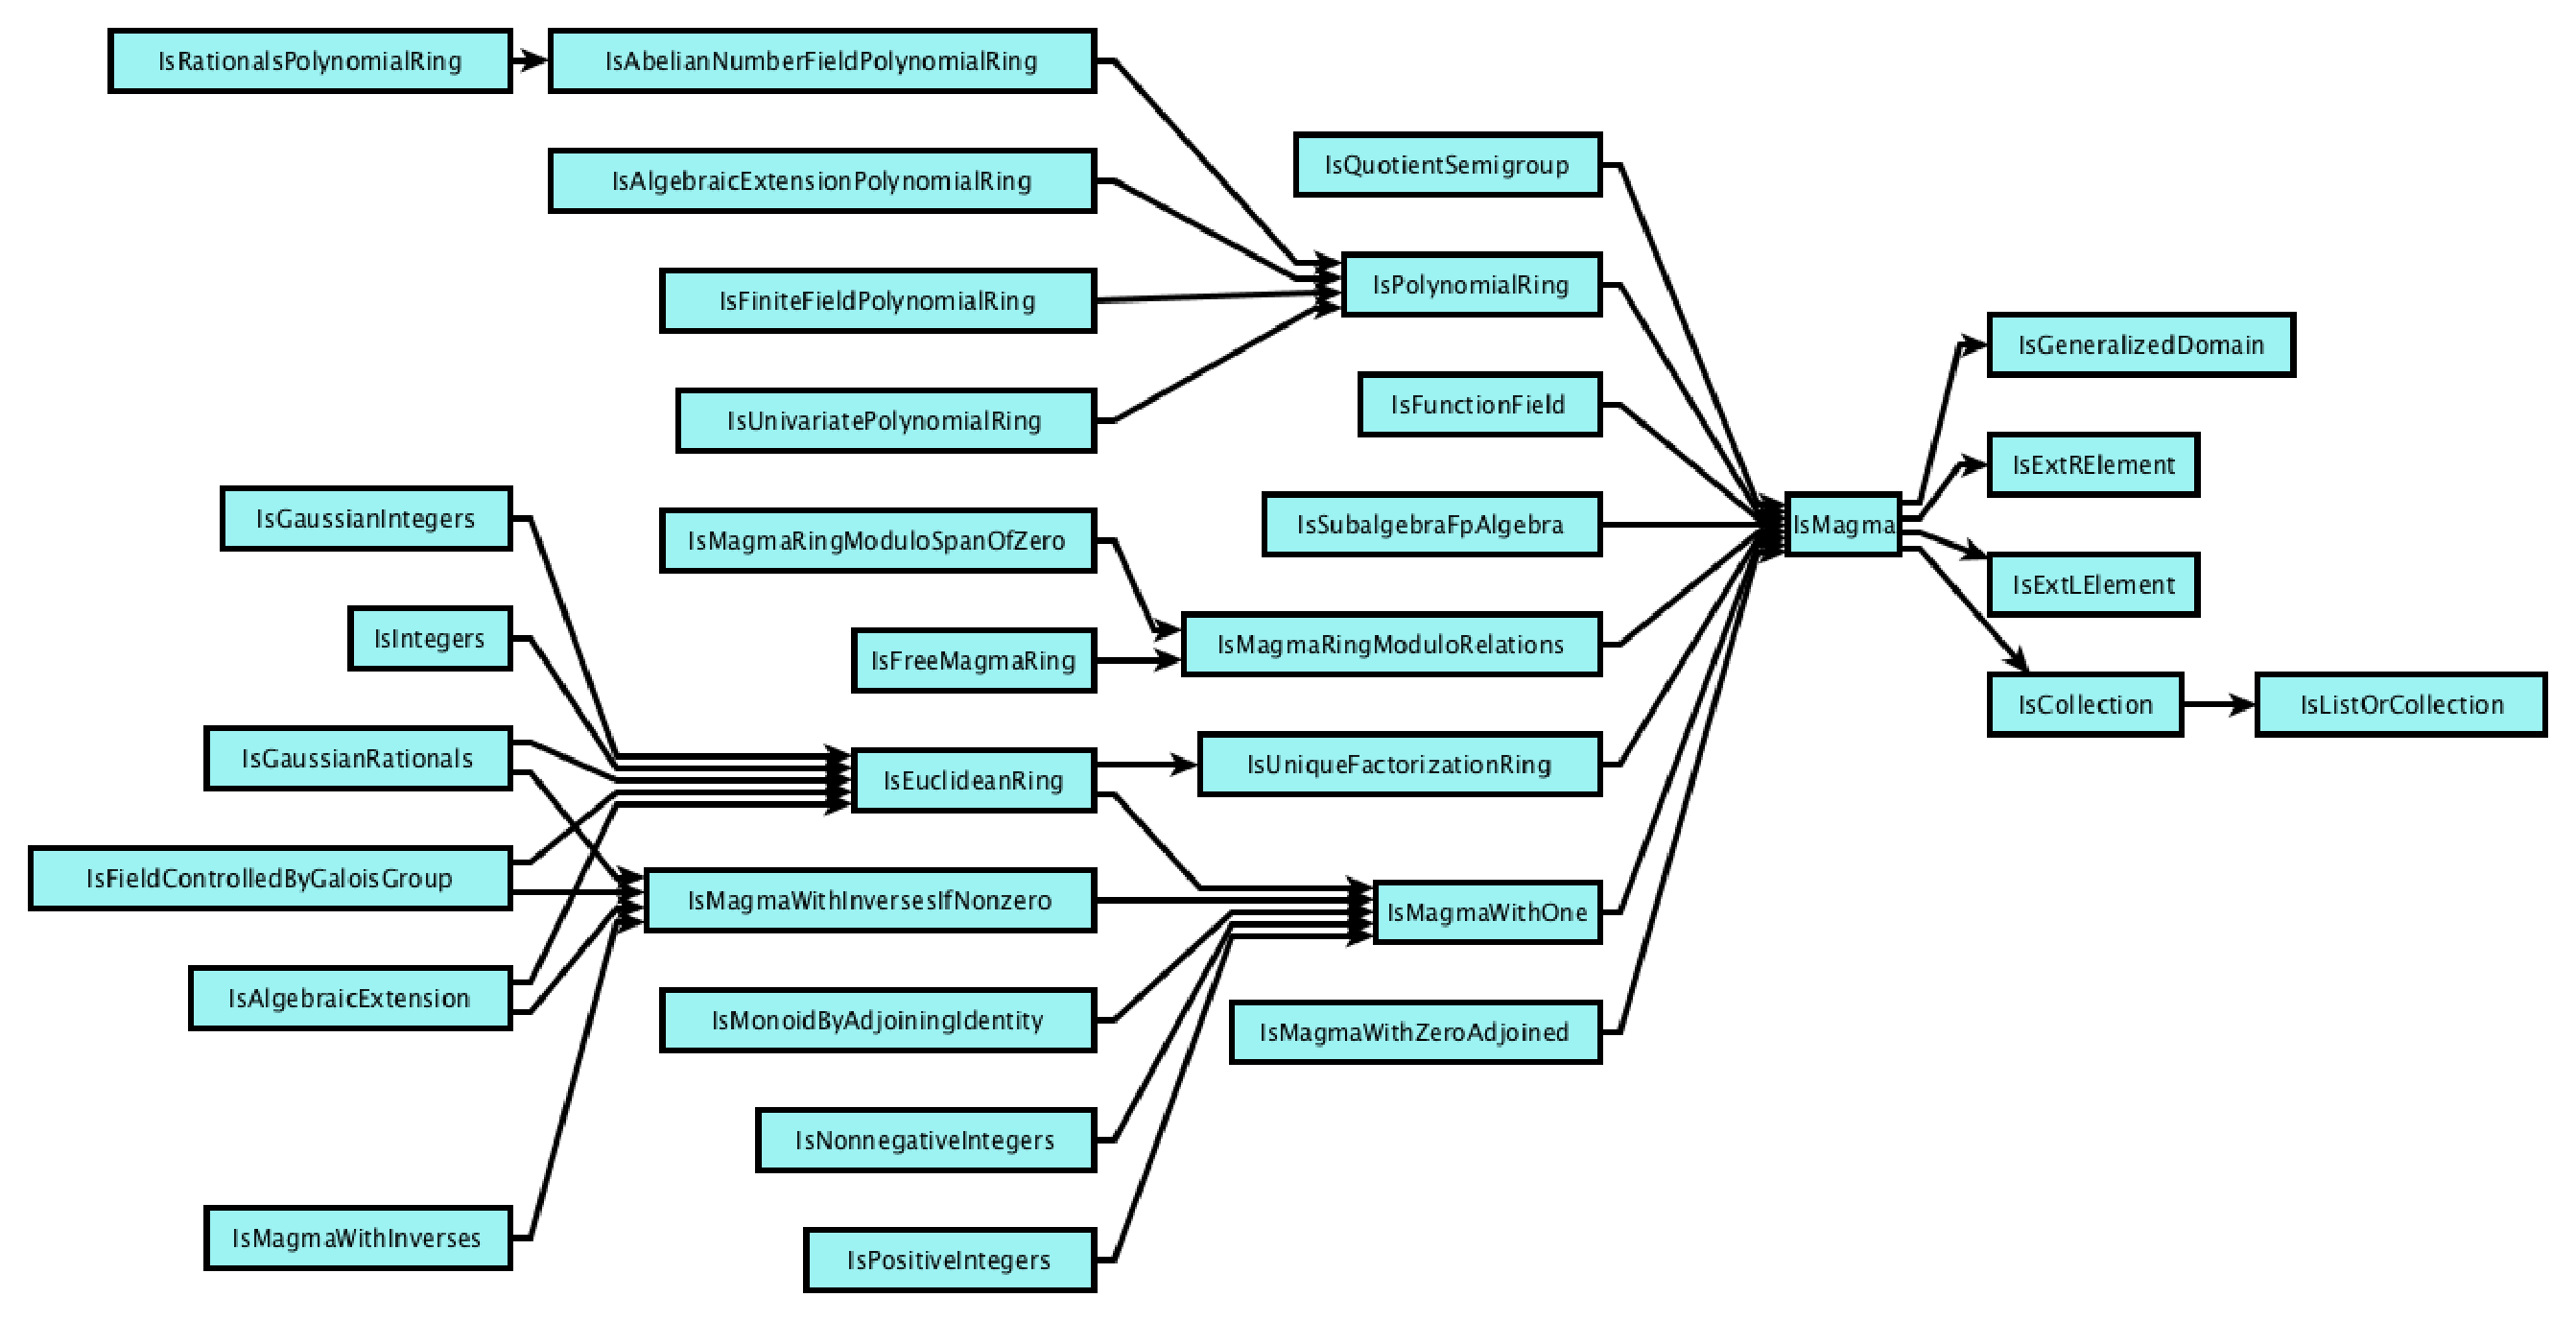
\includegraphics[width=\textwidth]{gap-ismagma}
  \caption{The \GAP Knowledge Graph (fragment).\label{fig:gap-ismagma}}
\end{figure}

As a side-effect of this work, we discovered quite a few inconsistencies in the \GAP
documentation which came from a semi-automated conversion of GAP manuals from the
\TeX-based manuals used in GAP 4.4.12 and earlier.  We developed the consistency checker
for the GAP documentation, which extracts type annotations from the documented GAP objects
and compares them with their actual types. It immediately reported almost 400
inconsistencies out of 3674 manual entries, 75\% of which have been
eliminated in the subsequent cleanup.

%%% Local Variables:
%%% mode: latex
%%% TeX-master: "paper"
%%% End:

%  LocalWords:  gapsage newpart texttt interop lst lstlisting Mehthod inparaenum behavior
%  LocalWords:  specializations ednote wrapfigure vspace mmt anncat formalized emph emph
%  LocalWords:  breuer-linton centering includegraphics gapdoc synchronized flexiformal
%  LocalWords:  lmfdb
